%%%%%%%%%%%%%%%%%%%%%%%%%%%%%%%%%%%%%%%%%%%%
% En 'includes.tex' se encuentran la importación de paquetes necesarios
%%%%%%%%%%%%%%%%%%%%%%%%%%%%%%%%%%%%%%%%%%%%
%%%%%%%%%%%%%%%%%%%%%%%%%%%%%%%%%%%%%%%%%
% University Assignment Title Page 
% LaTeX Template
% Version 1.0 (27/12/12)
%
% This template has been downloaded from:
% http://www.LaTeXTemplates.com
%
% Original author:
% WikiBooks (http://en.wikibooks.org/wiki/LaTeX/Title_Creation)
%
% License: CC BY-NC-SA 3.0 (http://creativecommons.org/licenses/by-nc-sa/3.0/)
% 
% Instructions for using this template:
% This title page is capable of being compiled as is. This is not useful for 
% including it in another document. To do this, you have two options: 
%
% 1) Copy/paste everything between \begin{document} and \end{document} 
% starting at \begin{titlepage} and paste this into another LaTeX file where you 
% want your title page.
% OR
% 2) Remove everything outside the \begin{titlepage} and \end{titlepage} and 
% move this file to the same directory as the LaTeX file you wish to add it to. 
% Then add \input{./title_page_1.tex} to your LaTeX file where you want your
% title page.
%
%%%%%%%%%%%%%%%%%%%%%%%%%%%%%%%%%%%%%%%%%
%\title{Title page with logo}
%----------------------------------------------------------------------------------------
%	PACKAGES AND OTHER DOCUMENT CONFIGURATIONS
%----------------------------------------------------------------------------------------
\PassOptionsToPackage{warn}{textcomp}
\documentclass[14pt]{extarticle}
%Paquetes para idioma español y codifcación UTF8
\usepackage[spanish]{babel}
\usepackage[utf8]{inputenc}
\usepackage{csquotes}

%%% BIBLATEX
\usepackage{biblatex}
%%% BIBLIOGRAPHY
\addbibresource{references.bib}

%fuente 'fourier'
\usepackage{fourier}
%paquete para URLs
\usepackage{url}
\usepackage[hidelinks]{hyperref}
%paquete para ubicar las imágenes
\usepackage{float}
%paquete para imágenes y en dónde las tiene que buscar
\usepackage{graphicx}
\graphicspath{{images/}}
%paquete para epígrafes
\usepackage{subcaption}
%paquete para definir los márgenes de la hoja
\usepackage[left=1.5cm,right=1.5cm,top=3cm,bottom=3cm]{geometry}
%paquete para poner todos y comentarios
\usepackage[colorinlistoftodos]{todonotes}
%paquete para trabajar con código
\usepackage{listings}
%paquete para trabajar con colores y definir propios
\usepackage{color}

%paquete para el checkmark y la cruz
\usepackage{pifont}
%paquete para el signo de copyright
\usepackage{textcomp}

%paquete para que los \texttt{} no rompan el margen de la página
\usepackage[htt]{hyphenat}

\usepackage{enumerate}
%paquete para armar layouts multicolumna
\usepackage{multicol}


%Cabeceras
\usepackage{fancyhdr}
\pagestyle{fancy}
\fancyhead[L]{Administración de Redes y Seguridad, 2018}
\fancyhead[C]{}
\fancyhead[R]{UNPSJB}

\fancyfoot[R]{Luciano Serruya Aloisi}

%Comando para poner doble comillas más fácil
\newcommand{\dq}[1]{``#1''}
\newcommand{\cmark}{\ding{51}}
\newcommand{\xmark}{\ding{55}}

\definecolor{comment-green}{rgb}{0,0.5,0}
\definecolor{bg-light-gray}{HTML}{E9E9E9}
\definecolor{bg}{HTML}{D0B698}

\lstdefinestyle{bashstyle}{
    language=Bash,
    backgroundcolor=\color{bg},
    basicstyle=\ttfamily,
  	keywordstyle=\bfseries\color{white},
    stringstyle=\color{blue},
    commentstyle=\color{comment-green}\itshape,
    numberstyle=\color{gray},
    identifierstyle=\color{black},
    rulecolor=\color{gray},
    showstringspaces=false,
    escapeinside={\%*}{*)},
    morekeywords={},
    otherkeywords={},
    breaklines=true,
    frame=trbl, 
    framexleftmargin=25pt,
    numbers=left,
    xleftmargin=\parindent,
    frameround=tttt,
    captionpos=b,
    % re tirado de los pelos, pero es lo que hay
    % sacado de:
    % https://tex.stackexchange.com/questions/24528/having-problems-with-listings-and-utf-8-can-it-be-fixed
    inputencoding=utf8,
    extendedchars=true,
    literate={á}{{\'a}}1 {é}{{\'e}}1 {í}{{\'i}}1 {ó}{{\'o}}1 {Ó}{{\'O}}1 {ú}{{\'u}}1,
}



\begin{document}

%%%%%%%%%%%%%%%%%%%%%%%%%%%%%%%%%%%%%%%%%%%%
% En 'titlepage.tex' se encuentra la página de título
%%%%%%%%%%%%%%%%%%%%%%%%%%%%%%%%%%%%%%%%%%%%
\begin{titlepage}

    \newcommand{\HRule}{\rule{\linewidth}{0.5mm}} % Defines a new command for the horizontal lines, change thickness here

    \center % Center everything on the page
     
    %----------------------------------------------------------------------------------------
    %	HEADING SECTIONS
    %----------------------------------------------------------------------------------------

    \textsc{\LARGE UNPSJB}\\[1cm] % Name of your university/college
    \textsc{\Large Licenciatura en Sistemas OPGCPI}\\[0.5cm] % Major heading such as course name
    \textsc{\large Administración de Redes y Seguridad}\\[0.5cm] % Minor heading such as course title

    %----------------------------------------------------------------------------------------
    %	TITLE SECTION
    %----------------------------------------------------------------------------------------

    \HRule \\[0.4cm]
    {\huge \bfseries Trabajo Práctico 1}\\[0.4cm] % Title of your document
    {\large \bfseries Concientización}\\[0.4cm] % Title of your document
    \HRule \\[1.5cm]
     
    %----------------------------------------------------------------------------------------
    %	AUTHOR SECTION
    %----------------------------------------------------------------------------------------


    \begin{minipage}[l]{0.5\textwidth}
        \begin{flushleft}
            \textbf{\textsf{Cátedra}}\\
            \large Lic. Bruno Damián Zappellini\\ 
            \linespread{4}
            \end{flushleft}
    \end{minipage}
    \begin{minipage}[l]{0.4\textwidth}
        \begin{flushright}
            \textbf{\textsf{Integrantes:}}\\
            \linespread{1}
            \large Luciano Serruya Aloisi\\
        \end{flushright}
    \end{minipage}\\[1.5cm]

    % If you don't want a supervisor, uncomment the two lines below and remove the section above
    %\Large \emph{Author:}\\
    %John \textsc{Smith}\\[3cm] % Your name

    %----------------------------------------------------------------------------------------
    %	DATE SECTION
    %----------------------------------------------------------------------------------------

    {\large \today}\\[1cm] % Date, change the \today to a set date if you want to be precise

    %----------------------------------------------------------------------------------------
    %	LOGO SECTION
    %----------------------------------------------------------------------------------------

    
\includegraphics[scale=1]{logoUnpsjb.png}\\[0.5cm] % Include a department/university logo - this will require the graphicx package
     
    %----------------------------------------------------------------------------------------

    % \vfill % Fill the rest of the page with whitespace

\end{titlepage}


%%%%%%%%%%%%%%%%%%%%%%%%%%%%%%%%%%%%%%%%%%%%
% INDICE
%%%%%%%%%%%%%%%%%%%%%%%%%%%%%%%%%%%%%%%%%%%%
\clearpage
\tableofcontents
\clearpage 

\lstset{style=bashstyle}

\section{Sistema de autenticación de SSH}

Según las páginas \texttt{man}, el comando \texttt{ssh-keygen} \emph{genera, gestiona, convierte, y autoriza claves para ssh. ssh-keygen puede generar claves para que las use SSH protocolo versión 2} 

\begin{figure}[H]
    \centering
    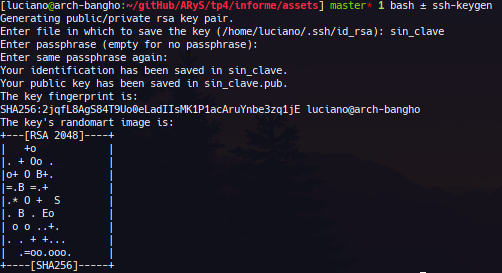
\includegraphics[scale=0.6]{images/ssh-sin-clave.png}
    \caption*{Creación de una llave SSH sin contraseña}
\end{figure}

\begin{figure}[H]
    \centering
    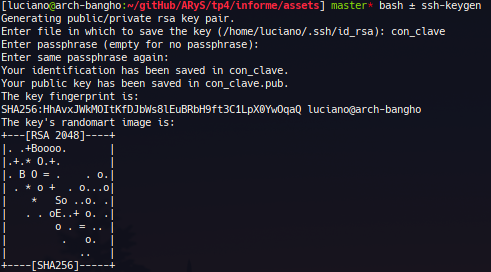
\includegraphics[scale=0.6]{images/ssh-con-clave.png}
    \caption*{Creación de una llave SSH con contraseña \dq{unaClave}}
\end{figure}

\subsection{Archivos de autorización}

Para gestionar el ingreso con \emph{clave pública} y para llevar registro de los sitios confiables a los cuales ya se ingresó, SSH mantiene dos archivos, respectivamente:

\begin{itemize}
    \item \emph{authorized\_keys}: lleva registro de las claves públicas aceptadas para conectarse vía SSH al sistema. Se podrán conectar con autenticación de clave pública sólo aquellos usuarios que tengan la correspondiente clave privada de la clave pública registrada en el archivo 
    \item \emph{known\_hosts}: indica a los sitios que se conectó el usuario y son seguros (antes de establecer la conexión SSH con un sitio nuevo, el sistema pregunta si desea confiar en el sitio) 
\end{itemize}

\subsection{Ingresando a un servidor remoto con clave pública}

Luego de registrar la clave pública personal en el servidor remoto y de haber configurado este último para que sólo permita ingresar (por SSH) mediante clave pública, se puede ingresar al servidor sin problemas.

Gracias al \emph{log} que imprime SSH al ejecutarlo con la bandera \texttt{-vvv}, se puede ver la siguiente sección con respecto al ingreso con clave pública

\begin{lstlisting}
.
.
.
debug1: Authentications that can continue: publickey
debug3: start over, passed a different list publickey
debug3: preferred publickey,keyboard-interactive,password
debug3: authmethod_lookup publickey
debug3: remaining preferred: keyboard-interactive,password
debug3: authmethod_is_enabled publickey
debug1: Next authentication method: publickey
.
.
.
\end{lstlisting}

\section{Túneles}

\subsection{Locales}

\emph{Ana es desarrolladora de aplicaciones web, y quiere probar algunos cambios con una base de datos de prueba que se encuentra en un servidor remoto. Ana no puede transferir la base de datos a su computadora, dado el excesivo tamaño de la misma. Sin embargo, Ana sabe que mediante la herramienta ssh puede hacer que su aplicación local utilice la base de datos remota} 
\vspace*{5mm}

La creación de un túnel SSH sería de igual manera para trabajar tanto con una base de datos MySQL como con una PostgreSQL, lo único que cambiaría es el puerto al cual redirigir la petición en el servidor remoto.

Lo primero a tener en cuenta es que Ana debe poder ingresar al servidor remoto vía SSH, ya sea teniendo un usuario y contraseña en el servidor, o habiendo instalado su clave pública. Luego, debe saber qué puerto utiliza su aplicación para conectarse a la base de datos local.

Suponiendo que la aplicación web de Ana utiliza el puerto 6060 para conectarse a la base de datos local, debería invocar SSH de la siguiente manera para crear un túnel:

\begin{itemize}
    \item MySQL: \texttt{ssh 6060:$<$IP\_SERVIDOR$>$:3306 $<$USUARIO\_ANA$>$@$<$IP\_SERVIDOR$>$} 
    \item PostgreSQL: \texttt{ssh 6060:$<$IP\_SERVIDOR$>:$5432 $<$USUARIO\_ANA$>$@$<$IP\_SERVIDOR$>$} 
\end{itemize}

\subsection{Remotos}

\emph{Matías tiene acceso a un servidor que escucha conexiones únicamente en el puerto 80, para las interfases de red físicas. Matías no puede alterar el firewall ya que no es administrador, sin embargo ha detectado que el servidor ejecuta un servicio SSH y no tiene restricciones para realizar conexiones salientes. Matías desea poder acceder al servidor SSH desde su computadora personal. Indique que con que argumentos debe invocar ssh desde el servidor (túnel reverso) para realizar la conexión desde su máquina personal} 
\vspace*{5mm}

En este caso, se necesita crear un túnel de tal forma que se pueda conectar la computadora personal de Matías con el servidor. Creando un túnel reverso \textbf{desde el servidor hacia la computadora personal} de Matías, el servidor abre un puerto en la computadora personal, redirigiendo todo el tráfico de ese puerto hacia un puerto propio del servidor.

Para crear el túnel reverso, se debe invocar SSH de la siguiente manera:

\begin{itemize}
    \item \texttt{ssh -R 2020:localhost:22 $<$USUARIO\_MATIAS$>$@$<$IP\_MATIAS$>$} 
\end{itemize}

Nótese que el uso del puerto 2020 es arbitrario, se podría utilizar cualquier puerto que no se esté usando en la PC de Matías. Luego, Matías se podrá conectar al servidor haciendo:

\begin{itemize}
    \item \texttt{ssh -p 2020 $<$USUARIO\_SERVIDOR$>$@$<$IP\_SERVIDOR$>$} 
\end{itemize}


\emph{Marina desea acceder a un servidor que administra José, pero ambos se encuentran detrás de un router que realiza network address translation (NAT).  Marina sabe que ambos pueden acceder a un tercer host. Indique qué comandos debe realizar Marina o José, para poder tener acceso ssh entre los servidores de los extremos} 
\vspace*{5mm}

Al igual que el escenario anterior, esta situación se puede resolver con un \textbf{túnel reverso}. 

Supóngase que Marina desea acceder a una aplicación web en el servidor de José, pero esta aplicación corre en el puerto 8080, y José no desea exponer los puertos de la máquina hacia afuera de la red. Teniendo José un acceso vía SSH al servidor público (el tercer host que se indica en el enunciado), puede crear el siguiente túnel reverso desde la máquina que corre la aplicación

\begin{itemize}
    \item \texttt{ssh -R 9000:localhost:8080 $<$USUARIO\_JOSE$>$@$<$IP\_SERVIDOR$>$} 
\end{itemize}

Ahora Marina podrá ingresar a la aplicación de José, navegando a la dirección \texttt{$<$IP\_SERVIDOR$>$:9000} 

\section{Aplicaciones con interfaz gráfica}

\emph{Ernesto sabe que en un servidor se está ejecutando el proceso X11. Desea ejecutar una aplicación gráfica remota (Por ej.: Firefox).  Describa que uso dio al cliente de ssh Ernesto}
\vspace*{5mm}

La bandera \texttt{-X} de SSH permite compartir el \emph{socket} de la instancia de X11 que se está corriendo en la máquina del cliente; de esta forma, se puede ejecutar una aplicación con interfaz gráfica en el servidor remoto (al cual se conectó mediante SSH), y ver la GUI en la máquina del cliente.  

\section{Archivos de configuración de conexiones}

Se desea confeccionar un archivo de configuración para manejar la siguiente conexión:

\begin{itemize}
    \item Se debe ejecutar con el comando \texttt{ssh servidor1} 
    \item Dirección IP: 192.168.1.40
    \item Nombre de usuario: \dq{administrador}
    \item Puerto de la conexión: 22022
    \item Autenticación por \emph{passphrase} desactivada 
    \item Utilizar la clave ubicada en \emph{\$HOME/.ssh/keys/servidor1} 
\end{itemize}

\begin{lstlisting}
Host servidor1
    # IP a la cual conectarse
    Host 192.168.1.40
    # Usuario con el cual conectarse
    User administrador
    # Puerto donde escucha SSH
    Port 22022
    # Desactivar passphrase
    BatchMode yes
    # Utilizar key particular
    IdentityFile ~/.ssh/keys/servidor1
\end{lstlisting}


\section{Direccionamiento de puertos dinámico}

Utilizando túneles locales o remotos, la intención es redirigir el tráfico de un puerto hacia un puerto de otra máquina. Si se desea redireccionar el tráfico de varias aplicaciones, se deben crear varios túneles. Esto resulta siendo tedioso y poco práctico.

Con el \textbf{direccionamiento de puertos dinámico} (\emph{\textbf{Dynamic port forwarding}}), se inicia un servidor de proxy que implementa el protocolo \textbf{SOCKS} para redirigir el tráfico automáticamente según el protocolo de aplicación del que se trate. 

Cabe aclarar lo siguiente, cuando se crea un túnel local o remoto, SSH no interpreta de ninguna manera el tráfico que fluye por el túnel; envía la información desde el puerto origen al puerto destino. Al crear un proxy SOCKS (con el parámetro de SSH \texttt{-D}), SSH actúa como un servidor proxy, manejando conexiones de varios puertos distintos (necesita interpretar el tráfico para determinar el puerto destino) \autocite{SODynamicPortForwarding}

\subsection{Configuración de Firefox para usar un proxy SOCKS}

\begin{enumerate}
    \item Iniciar el servidor de proxy con la siguiente línea de SSH
    \begin{itemize}
        \item \texttt{ssh -D $<$PUERTO$>$ $<$USUARIO$>$@$<$HOST$>$} 
    \end{itemize}
    \item En Firefox, ir a \texttt{Edit} \textrightarrow \texttt{Preferences}  
    \item Dirigirse a la sección de \texttt{Network Proxy} \textrightarrow \texttt{Setings...} 
    \item Tildar \texttt{Manual proxy configuration} 
    \item Borrar todos los campos texto, y en el campo de \texttt{SOCKS Host}, ingresar
    \begin{itemize}
        \item \texttt{127.0.0.1}, Puerto \texttt{1080}  
    \end{itemize}
\end{enumerate}

Al utilizar el navegador con el proxy SOCKS configurado, las peticiones que realiza el navegador no tendrán como IP de origen la máquina en la cual está corriendo el navegador, sino que su IP origen será la de la máquina que esté corriendo el servidor proxy.

\vspace*{5mm}

La red TOR\footnote{Programa que protege y hace anónima la comunicación por Internet \autocite{TOR}} utiliza servidores de proxy SOCKS para hacer la navegación por Internet anónima; cada petición pasa por tres servidores de proxy distintos antes de llegar a destino













%%%%%%%%%%%%%%%%%%%%%%%%%%%%%%%%%%%%%%%%%%%%
% FIN DOCUMENTO, AHORA REFERENCIAS
%%%%%%%%%%%%%%%%%%%%%%%%%%%%%%%%%%%%%%%%%%%%
\clearpage
\printbibliography

\end{document}
